\documentclass[a4paper, 12pt]{article} % тип документа

%%%Библиотеки
	%\usepackage[warn]{mathtext}	
	\usepackage[T2A]{fontenc}   %Кодировка
	\usepackage[utf8]{inputenc} %Кодировка исходного текста
	\usepackage[english, russian]{babel} %Локализация и переносы
	\usepackage{caption}
	\usepackage{listings}
	\usepackage{amsmath, amsfonts, amssymb, amsthm, mathtools}
	\usepackage[warn]{mathtext}
	\usepackage[mathscr]{eucal}
	\usepackage{wasysym}
	\usepackage{graphicx} %Вставка картинок правильная
	\DeclareGraphicsExtensions{.pdf,.png,.jpg}
	\graphicspath{ {images/} }
	
	\setlength{\parskip}{0.5cm}
	
	\usepackage{pgfplots}
	\usepackage{indentfirst}
	\usepackage{float}    %Плавающие картинки
	\usepackage{wrapfig}  %Обтекание фигур (таблиц, картинок и прочего)
	\usepackage{fancyhdr} %Загрузим пакет
	\usepackage{lscape}
	\usepackage{xcolor}
	\usepackage[normalem]{ulem}
	\usepackage{wasysym}
	\usepackage{subfig}
	\usepackage{graphicx}
	
	\usepackage{titlesec}
	\titlelabel{\thetitle.\quad}

	\usepackage{hyperref}
	\newenvironment{comment}{}{}

%%%Конец библиотек

%%%Настройка ссылок
%%%	\hypersetup
%%%	{
%%%		colorlinks = true,
%%%		linkcolor  = blue,
%%%		filecolor  = magenta,
%%%		urlcolor   = blue
%%%	}
%%%Конец настройки ссылок


%%%Настройка колонтитулы
    \pagestyle{fancy}
    \fancyhead{}
    \fancyhead[L]{1.1.1}
    \fancyhead[R]{Засимов Георгий, группа Б01-109}
    \fancyfoot[C]{\thepage}
%%%конец настройки колонтитулы



\usepackage[T2A]{fontenc}			% кодировка
\usepackage[utf8]{inputenc}			% кодировка исходного текста
\usepackage[english,russian]{babel}	% локализация и переносы
\usepackage{tikz}
\usepackage{pgfplots}


% Математика
\usepackage{amsmath,amsfonts,amssymb,amsthm,mathtools} 


\usepackage{wasysym}

\begin{document}

%%%Начало титульника
\begin{titlepage}

    \newpage
    \begin{center}
        \normalsize Московский физико-технический институт \\(национальный исследовательский университет)
    \end{center}

    \vspace{6em}

    \begin{center}
        \Large Лабораторная работа по общему курсу физики\\
    \end{center}

    \vspace{1em}

    \begin{center}
        \Large \textbf{Отчёт о выполнении лабораторной работы 1.4.1\\ {Изучение экспериментальных погрешностей на примере физического маятника}}
    \end{center}

    \vspace{2em}

    \begin{center}
        \large Засимов Георгий Алексеевич \\
        Группа Б01-109
    \end{center}

    \vspace{\fill}

    \begin{center}
    Долгопрудный \\2021
    \end{center}
    
\end{titlepage}
%%%Конец Титульника

\newpage

%\\\\\\\\\\\\\\\\\\\\\\\\\\\\\\\\\\\\\\\\\\\\\\\\\\\\\\\\\\\\\\\\\\\\
\section* {1. Аннотация}

    В работе исследуются свободные колебания физического маятника. Определяются периоды колебаний маятника в зависимости от расстояния между точкой подвеса и центром масс. По результатам измерений определяется ускорение свободного падения. Сравниваются значения, полученные как среднее по результатам пробных измерений и серии измерений, а также при помощи метода наименьших квадартов.

%\\\\\\\\\\\\\\\\\\\\\\\\\\\\\\\\\\\\\\\\\\\\\\\\\\\\\\\\\\\\\\\\\\\\\
\section* {2. Теоретические сведения и методика измерений}

    Физический маятник - это любое твердое тело, которое под действием силы тяжести может свободно качаться вокруг неподвижной горизонтальной оси (острое ребро опорной призмы - ось качания маятника); другими словами, это совокупность жестко связанных точечных масс.\\ 
    
\begin{center}
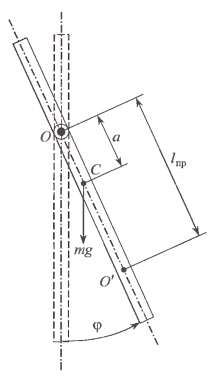
\includegraphics[width=4cm, height=7cm]{phys_mayat}
\end{center}

\begin{flushright}
{\scriptsize \textbf{Рис 1.} \textbf {Физический маятник}}
\end{flushright}

    
    В данной работе в качестве физического маятника (рис. 1)
    используется однородный стальной стержень длиной l. На
    стержне закрепляется опорная призма, острое ребро которой
    является осью качания маятника.\\
    Призма не перемещается, а дополнительный груз, закрепленный на стержне перемещается вдоль него, меняя таким образом центр масс системы. Момент инерции маятника будет зависеть от положения груза относиттельно оси каачания (см рис 2).\\
    
\begin{center}
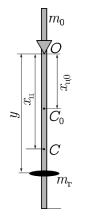
\includegraphics[width=4cm, height=8cm]{phys_mayat_2}
\end{center}

\begin{flushright}
{\scriptsize \textbf{Рис 2.} \textbf {Физический маятник с грузом}}
\end{flushright}
    
    Положение центра масс маятника вычисляется по формуле:

\begin{equation} \label{центр масс}
    x_{c} = \frac{m_{0}x_{c_0} + m_{r}y}{M}
\end{equation}


    Момент инерции стержня массой m, длины l, если ось вращения проходит на расстоянии а от центра масс по теореме Гюйгенса-Штейнера вычисляется по формуле:
    
\begin{equation} \label{момент инерции}
    J = \frac{ml^2}{12} + ma^2
\end{equation}

    Период колебаний произвольного физического маятника находим по формуле:
    
\begin{equation} \label{период}
    T = 2\pi\sqrt{\frac{J}{m g a}}
\end{equation}

    А период колебаний произвольного физического маятника со стержнем длины l, аодвешенного  на расстоянии a от центра:
    
\begin{equation} \label{период с а}
    T = 2\pi\sqrt{\frac{\frac{l^2}{12} + a^2}{g a}}
\end{equation}

    Вычислить положение центра масс груза можно по формуле:
   
\begin{equation} \label{центр масс груза}
    y = \frac{M x_{c} - m_0x_{c_0}}{m_r}
\end{equation}

    Период колебаний для маятника с грузом:

\begin{equation}\label{период с грузом}
    T = 2\pi\sqrt{\frac{J_0 + m_r y^2}{g M x_c}}
\end{equation}


%\\\\\\\\\\\\\\\\\\\\\\\\\\\\\\\\\\\\\\\\\\\\\\\\\\\\\\\\\\\\\\\\\\\\\\
\section*{3. Оборудование и экспериментальные погрешности}

    Погрешности приборов: $\delta $ линейки = 0.5 мм\\
    $\delta $ секундомера = 0.1 с (погрешность округления прибора)\\
    $\delta $ округления электронных весов = 0.05 г\\


%\\\\\\\\\\\\\\\\\\\\\\\\\\\\\\\\\\\\\\\\\\\\\\\\\\\\\\\\\\\\\\\\\\\\\\
\section*{4. Результаты измерений и обработка данных}

\subsection*{4.1. Оценка погрешностей}

    Относительная погрешность измерения длин:
    
\[
    \varepsilon_{max} = \frac{0,5}{500} = 0,1\% 
\]

    Используемые в работе инструменты позволяют вести измерения длин
    с точностью вплоть до 0,1\%. Для получения конечного результата с данной точностью период колебаний следует измерять с той же относительной погрешностью: не хуже, чем $\varepsilon\sim0,1\%$.
    
    Результаты измерений масс сотавляющих маятника ($m_{1}, m_{2}, m_{3}$ - стержня, призмы, груза) и длины стержня (l) с погрешностями:
    
\[
    m_{1} = 1019,20 \pm 0,05 g  \quad  (\varepsilon_{1} = 0,005\%)
\]
\[
    m_{2} = 72,30 \pm 0,05 g  \quad   (\varepsilon_{2} = 0,07\%)
\]
\[
    m_{3} = 372,50 \pm 0,05 g  \quad   (\varepsilon_{3} = 0,013\%)
\]
\[
    l  = 50 \pm 0,005 mm  \quad   (\varepsilon_l = 0,01\%)
\]
    Измерим расстояние от опорной призмы до центра масс стержня $x_{c_0}$ = 30,5 см. ($\varepsilon_{c_0} = 0,016\%$).
    
    Проведём пробные колебания (без груза, n = 20 колебаний, расстояние от центра масс стержня до опорной призмы а = 30,5 см, см результаты в таблице 1) для определения предварительного хначения ускорения свободного падения, а также для вычислени необходимого и достаточного количества измеряемых периодов колебаний для получения необходимой погрешности. Так как мы будем строить график зависимости u от v, где u = $T^2xц$, v = $a^2$. Чтобы погрешность измерения периода Т не влияла на итоговую погрешность, необходимо, чтобы погрешность $T^2$ не превышала $0,1\%$ - погрешность измерения центра масс стержня. Для этого найдём относительную погрешность округления счетчика периодов $\delta_{отн}\frac{0,01}{1,525} \approx 0,7\%$. Где $T_1 = T_2 = T_3 = 1,525$ c - период пробных колебаний, $0,01 с$ - погрешность округления счетчика. Вычислим необходимое количество измерений периодов в последующих измерениях. Погрешность $T^2 \approx 0,05\%$: $n = 26$ шт. 

   
\begin{table}[H]
\centering
\begin{tabular}{|l|l|l|l|}
\hline
    №    & 1    & 2    & 3    \\ \hline
    t, c & 30,5 & 30,5 & 30,5 \\ \hline
    T, c & 1,525 & 1,525 & 1,525 \\ \hline
\end{tabular}
\end{table}

\begin{flushright}
{\scriptsize \textbf{Таблица 1.} \textbf {Результаты пробных измерений.}}
\end{flushright}

    Рассчитаем погрешность измерения времени, так как все 3 измеренные величины совпадают, то полная погрешность измерения времени равна её систематической составляюющей $\delta = 0,01 c$. $\varepsilon_t = 0,003\%$.

    Полученное предварительное значение $g$ из формулы \eqref{период с а} $g \approx 9,81$ м/$c^2$. Полученное значение совпадает с табличным значением.\\


\subsection*{4.2. Обработка результатов}

    Представим полученные результаты основных измерений в Таблице 2. 
    Рассчитаем среднее занчение ускорения свободного падения $g = 9,6 \pm 0,5$ м/$c^2$.
    Погрешности при нахождении $J$:

\[\varepsilon_{J} = \sqrt{4 \frac{\sigma_{lin}^2}{x_{c}^2}} = 0,3\%\]

    Найдем среднее значение $g = 9,72$ м/$c^2$.
    Найдем погрешность измерения g:
    
    \[\varepsilon_{g} = \sqrt{\varepsilon_{J}^2 + \varepsilon_{t}^2 + \varepsilon_{lin}^2 + 4\varepsilon_{c}^2} = 1,3\%\]
    
    
\begin{table}[H]
\centering
\begin{tabular}{|l|l|l|l|l|l|l|l|}
\hline
№  & y, м & хц, м & t1, c & t2, c & t3, c & T, c   & g \\ \hline
1  & 0,47 & 0,350 & 39,24 & 39,23 & 39,23 & 1,5090 & 9,356     \\ \hline
2  & 0,18 & 0,272 & 36,97 & 36,97 & 36,97 & 1,4219 & 9,895     \\ \hline
3  & 0,17 & 0,269 & 37,06 & 37,05 & 37,06 & 1,4253 & 9,882     \\ \hline
4  & 0,31 & 0,306 & 37,36 & 37,36 & 36,36 & 1,4241 & 9,828     \\ \hline
5  & 0,31 & 0,305 & 37,03 & 37,02 & 37,02 & 1,4240 & 9,823     \\ \hline
6  & 0,42 & 0,335 & 38,5  & 38,5  & 38,49 & 1,4806 & 9,435     \\ \hline
7  & 0,39 & 0,329 & 38,26 & 38,26 & 38,26 & 1,4715 & 9,4570    \\ \hline
8  & 0,59 & 0,380 & 38,05 & 38,09 & 38,07 & 1,4642 & 10,6888   \\ \hline
9  & 0,36 & 0,320 & 37,88 & 37,88 & 37,88 & 1,4569 & 9,524     \\ \hline
10 & 0,49 & 0,355 & 39,5  & 39,5  & 39,5  & 1,5192 & 9,332     \\ \hline
\end{tabular}
\end{table}

\begin{flushright}
{\scriptsize \textbf{Таблица 3.} \textbf {Результаты основной измерений эксперимента.}}
\end{flushright}

    Построим график завимости периода колебаний Т от смещения груза а (погрешность измерения периода мала, её мы не учитываем при построении графика). 

\begin{center}
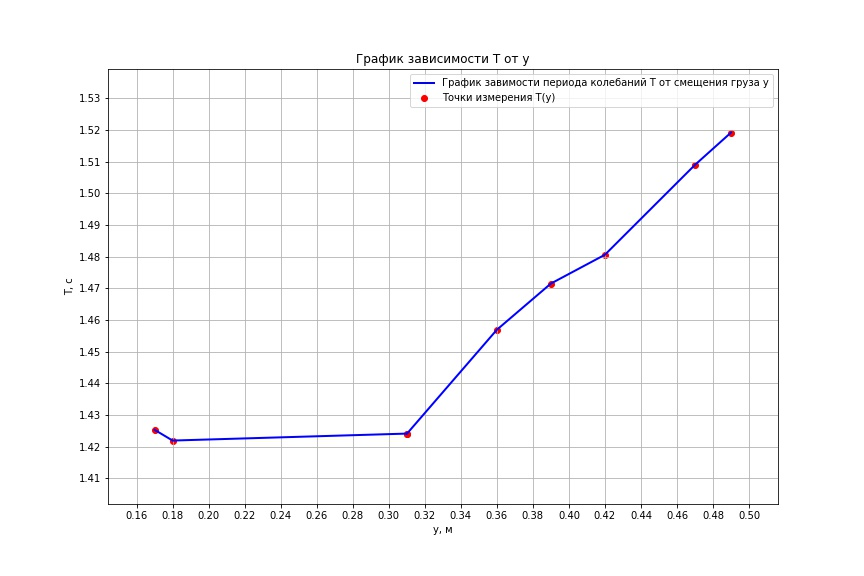
\includegraphics[width=15cm, height=8cm]{graph_1.jpg}
\end{center}

\begin{flushright}
{\scriptsize \textbf{Рис 3.} \textbf {График зависимости периода колебаний от расстояния между точкой подвеса и центром масс маятника.}}
\end{flushright}

    Убедимся, что полученная зависимость имеет минимум - T = 1,4241 c при значении у = 0,309 м.\\


    
    Посторим график зависимости v от u, где $v = y^2$, $u = T^2x_c$.



\begin{center}
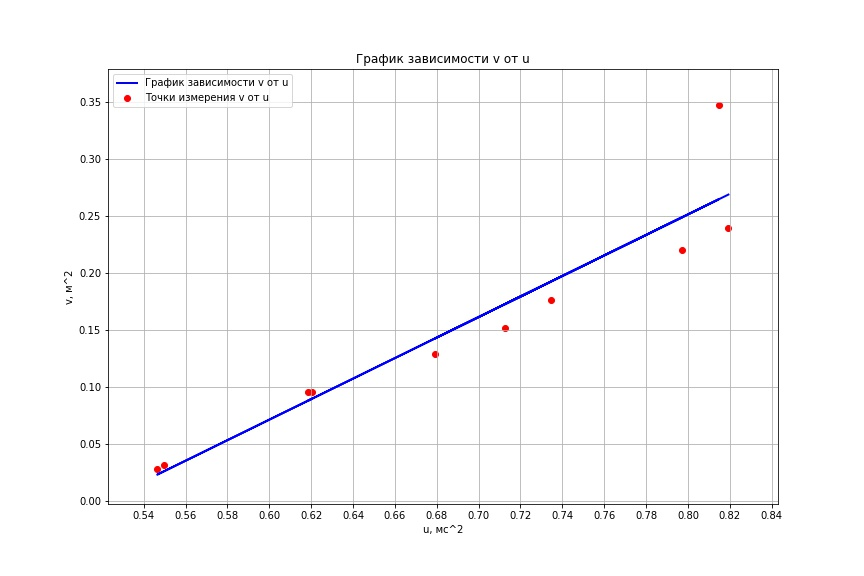
\includegraphics[width=15cm, height=9cm]{graph_2.jpg}
\end{center}

\begin{flushright}
{\scriptsize \textbf{Рис 4.} \textbf {График зависимости квадрата расстояния между точкой подвеса и ценром масс маятника от $T^2x_c$ (Т - период колебаний маятника, $x_c$ - расстояние от точки подвеса до центра масс стержня.}}
\end{flushright}

    Погрешность измерения $x_c$:
    
\[\sigma_{x_c} = \sqrt{\left(\frac{\Delta x}{x_c}\right)^2 + \left(2\frac{\Delta T}{T}\right)^2} = 0,2 m/c^2\]\\\\

    Значение $g$ по формуле \eqref{период с грузом}:
    
\[g = 9,72 \pm 0,13 m/c^2\]


    Построим аппроксимирующую прямую. Найдём хначение $k$ по методу наименьших квадратов для линейной зависимости.
    
\[k = \frac{<xy> - <y><x>}{<x^2> - <x>^2} = 0,9\]    
    
    Погрешность определения значения k:
    
\[\sigma_{k}^{oc} = \sqrt{\frac{1}{N-1} \left(\frac{<y^2> - <y>^2}{<x^2> - <x>^2} - k^2\right)} = 0,32\]


    Итоговая погрешность вычисления $g$ при помощи $k$:
    
\[\sigma_{ov} = \sqrt{\sigma_{xc}^2 + \sigma_k^2} =  0,38 m/c^2\]


    Ускорение свободного падения по значению k:
    
\[g_{mnk} = 11,7 \pm  0,4 m/c^2\]

\[\varepsilon_{g_{mnk}} = 3,4\%\]



%\\\\\\\\\\\\\\\\\\\\\\\\\\\\\\\\\\\\\\\\\\\\\\\\\\\\\\\\\\\\\\\\\\\\\\\
\newpage
\section*{5. Обсуждение результатов и выводы}

    В ходе проведения работы были получены значения ускорения свободного падения, в пробном эксперименте:
    
    $g = 9,81 \pm 0,01$ м/$c^2$ $\varepsilon_g = 0,1\%$\\
    
    и в ходе основной серии измерений по формуле для периода колебаний физического маятника с грузом:
    
    $\overline{g} = 9,72 \pm 0,13$ м/$c^2$ $\varepsilon_g = 1,3\%$\\
    
    
    Cравним полученные значения со значением $g$, полученным при помощи метода наименьших квадратов: 
    
    $g = 11,7 \pm 0,4 $ м/$c^2$ $\varepsilon_g = 3,4\%$\\
    
    Значение $g$, полученное при помощи метода наименьших квадратов сильнее отличается от табличного значения (в пределах $4\sigma$). Данное отклонение связано с учетом погрешности нахождения коэффициента угла наклона аппроксимирующей прямой графика зависимости $v$ от $u$.

    Данные значения отличаются от табличного $(g = 9,81 m/c^2)$ в пределах $2\sigma$. Имеющиеся расхождения можно объяснить тем,что при расчетах не учитывалась масса опорной призмы, которая влияет на положение центра масс маятника и как следствие на значение момента инерции и результат.

\end{document}


%\\\\\\\\\\\\\\\\\\\\\\\\\\\\\\\\\\\\\\\\\\\\\\\\\\\\\\\\\\\\\\\\\\\\\\\\\\\\\\\\\\\\\\\\\\\\\\\\\\\\\\\\\\\\\\\\\\\\\\\\\\\\\\\\\\\\\\\\\\\\\\\\\\\\\\\\\\\\\\\\\\\\\\\\\\\\\\\\\\\\\\\\\\\\\\\\\\\\\\\\\\\\\\\\\\\\\\\\\\\\\\\\\\\\\\\\\\\\\\

